
%%%%%%%%%%%%%%%%%%%%%%%%%%%%%%%%%%%%%%%%%%%%%%%%%%%%%%%%%%%%%%%%%%%%%%%%%%%%%%%%%%%%%%%%%%%%%%%%%
%
% Document:      DM  organisation chart reporting lines
%
%%%%%%%%%%%%%%%%%%%%%%%%%%%%%%%%%%%%%%%%%%%%%%%%%%%%%%%%%%%%%%%%%%%%%%%%%%%%%%

\documentclass{article}

\usepackage{times,layouts}
\usepackage{tikz,hyperref,amsmath}
\usetikzlibrary{positioning,arrows,shapes,decorations.shapes,shapes.arrows}
\usetikzlibrary{backgrounds,calc}

\usepackage[paperwidth=30cm,paperheight=20.0cm,
left=-2mm,top=3mm,bottom=0mm,right=0mm,
noheadfoot,marginparwidth=0pt,includemp=false ]{geometry}


\newcommand\showpage{%
\setlayoutscale{0.5}\setlabelfont{\tiny}\printheadingsfalse\printparametersfalse
\currentpage\pagedesign}

\hypersetup{pdftitle={DM organisation }, pdfsubject={Diagram illustrating the
 reporting lines in LSST DM Group}, pdfauthor={ William O'Mullane}}


%%%%%%%%%%%%%%%%%%%%%%%%%%%%%%%%%%%%%%%%%%%%%%%%%%%%%%%%%%%%%%%%%%%%%%%%%%%%%%%%%%%%%%%%%%%%%%%%%
%
% Document:      Boxes and lines for all diagrams
%
%%%%%%%%%%%%%%%%%%%%%%%%%%%%%%%%%%%%%%%%%%%%%%%%%%%%%%%%%%%%%%%%%%%%%%%%%%%%%%

\tikzstyle{divbox}=[rectangle, rounded corners=3pt, draw=blue, top color=blue!30!white, bottom
color=white, very thick, minimum height=12mm, inner sep=3pt, text centered, text width=35mm]

\tikzstyle{arcbox}=[rectangle, rounded corners=3pt, draw=red, top color=yellow!50!white, bottom
color=white, very thick, minimum height=12mm, inner sep=2pt, text centered, text width=50mm]

\tikzstyle{psbox}=[rectangle, rounded corners=3pt, draw=red, top color=green!50!white, bottom
color=cyan, very thick, minimum height=10mm, inner sep=2pt, text centered, text width=35mm]

\tikzstyle{pobox}=[rectangle, rounded corners=3pt, draw=red, top color=blue!50!white, bottom
color=cyan, very thick, minimum height=10mm, inner sep=2pt, text centered, text width=35mm]

\tikzstyle{docbox}=[rectangle, rounded corners=3pt, draw=black, fill=cyan!50!white, 
 very thick, minimum height=12mm, inner sep=2pt,  text centered, text width=30mm]

\tikzstyle{docboxm}=[rectangle, rounded corners=3pt, draw=black, fill=red!50!white, 
 very thick, minimum height=12mm, inner sep=2pt,  text centered, text width=30mm]

\tikzstyle{docboxicd}=[rectangle, rounded corners=3pt, draw=black, fill=green!70!white, 
 very thick, minimum height=12mm, inner sep=2pt,  text centered, text width=30mm]

\tikzstyle{gbox}=[rectangle, rounded corners=3pt, draw=orange!80!black, top color=orange!30!white,
bottom color=white, very thick, minimum height=12mm, inner sep=5pt, text badly ragged, text width=40mm]

\tikzstyle{mbox}=[rectangle, rounded corners=3pt, draw=blue, top color=cyan!50!white, bottom
color=white, very thick, minimum height=8mm, inner sep=2pt, text centered, text width=30mm]

\tikzstyle{line}=[-, thick]
\tikzstyle{sline}=[-, thick, dashed, olive]
\tikzstyle{dline}=[->, thick, cyan]
\tikzstyle{tline}=[->, thick, dashed, blue]
\tikzstyle{pline}=[->, thick,  black!60!white]

\xdefinecolor{softviolet}{rgb}{0.85, 0.8, 1.0}




\newcommand\dmmnode[6][]{
            \node (#2) [mbox, text width=36mm, rectangle split, rectangle split parts=2, #1]
                {
                \strut #3
                \nodepart{second} \vspace{39mm}
                };
             \node({#2}t) [mbox,minimum height=9mm, below=8mm of {#2}.north, text width=32mm] {\parbox[height=6mm]{0pt}{}{\small \bf Manager }\\\strut#4};
             \node({#2}s) [#6,minimum height=9mm, below=2pt of {#2}t, text width=32mm] {{\small \bf Product Owner}\\\strut#5};
        }

\newcommand\dmnode[6][]{
            \node (#2) [mbox, text width=36mm, rectangle split, rectangle split parts=2, #1]
                {
                \strut #3
                \nodepart{second} \vspace{39mm}
                };
             \node({#2}t) [mbox,minimum height=9mm, below=8mm of {#2}.north, text width=32mm] {\parbox[height=6mm]{0pt}{}{\small \bf T/CAM}\\\strut#4};
             \node({#2}s) [#6,minimum height=9mm, below=2pt of {#2}t, text width=32mm] {{\small \bf Product Owner}\\\strut#5};
        }


\begin{document}

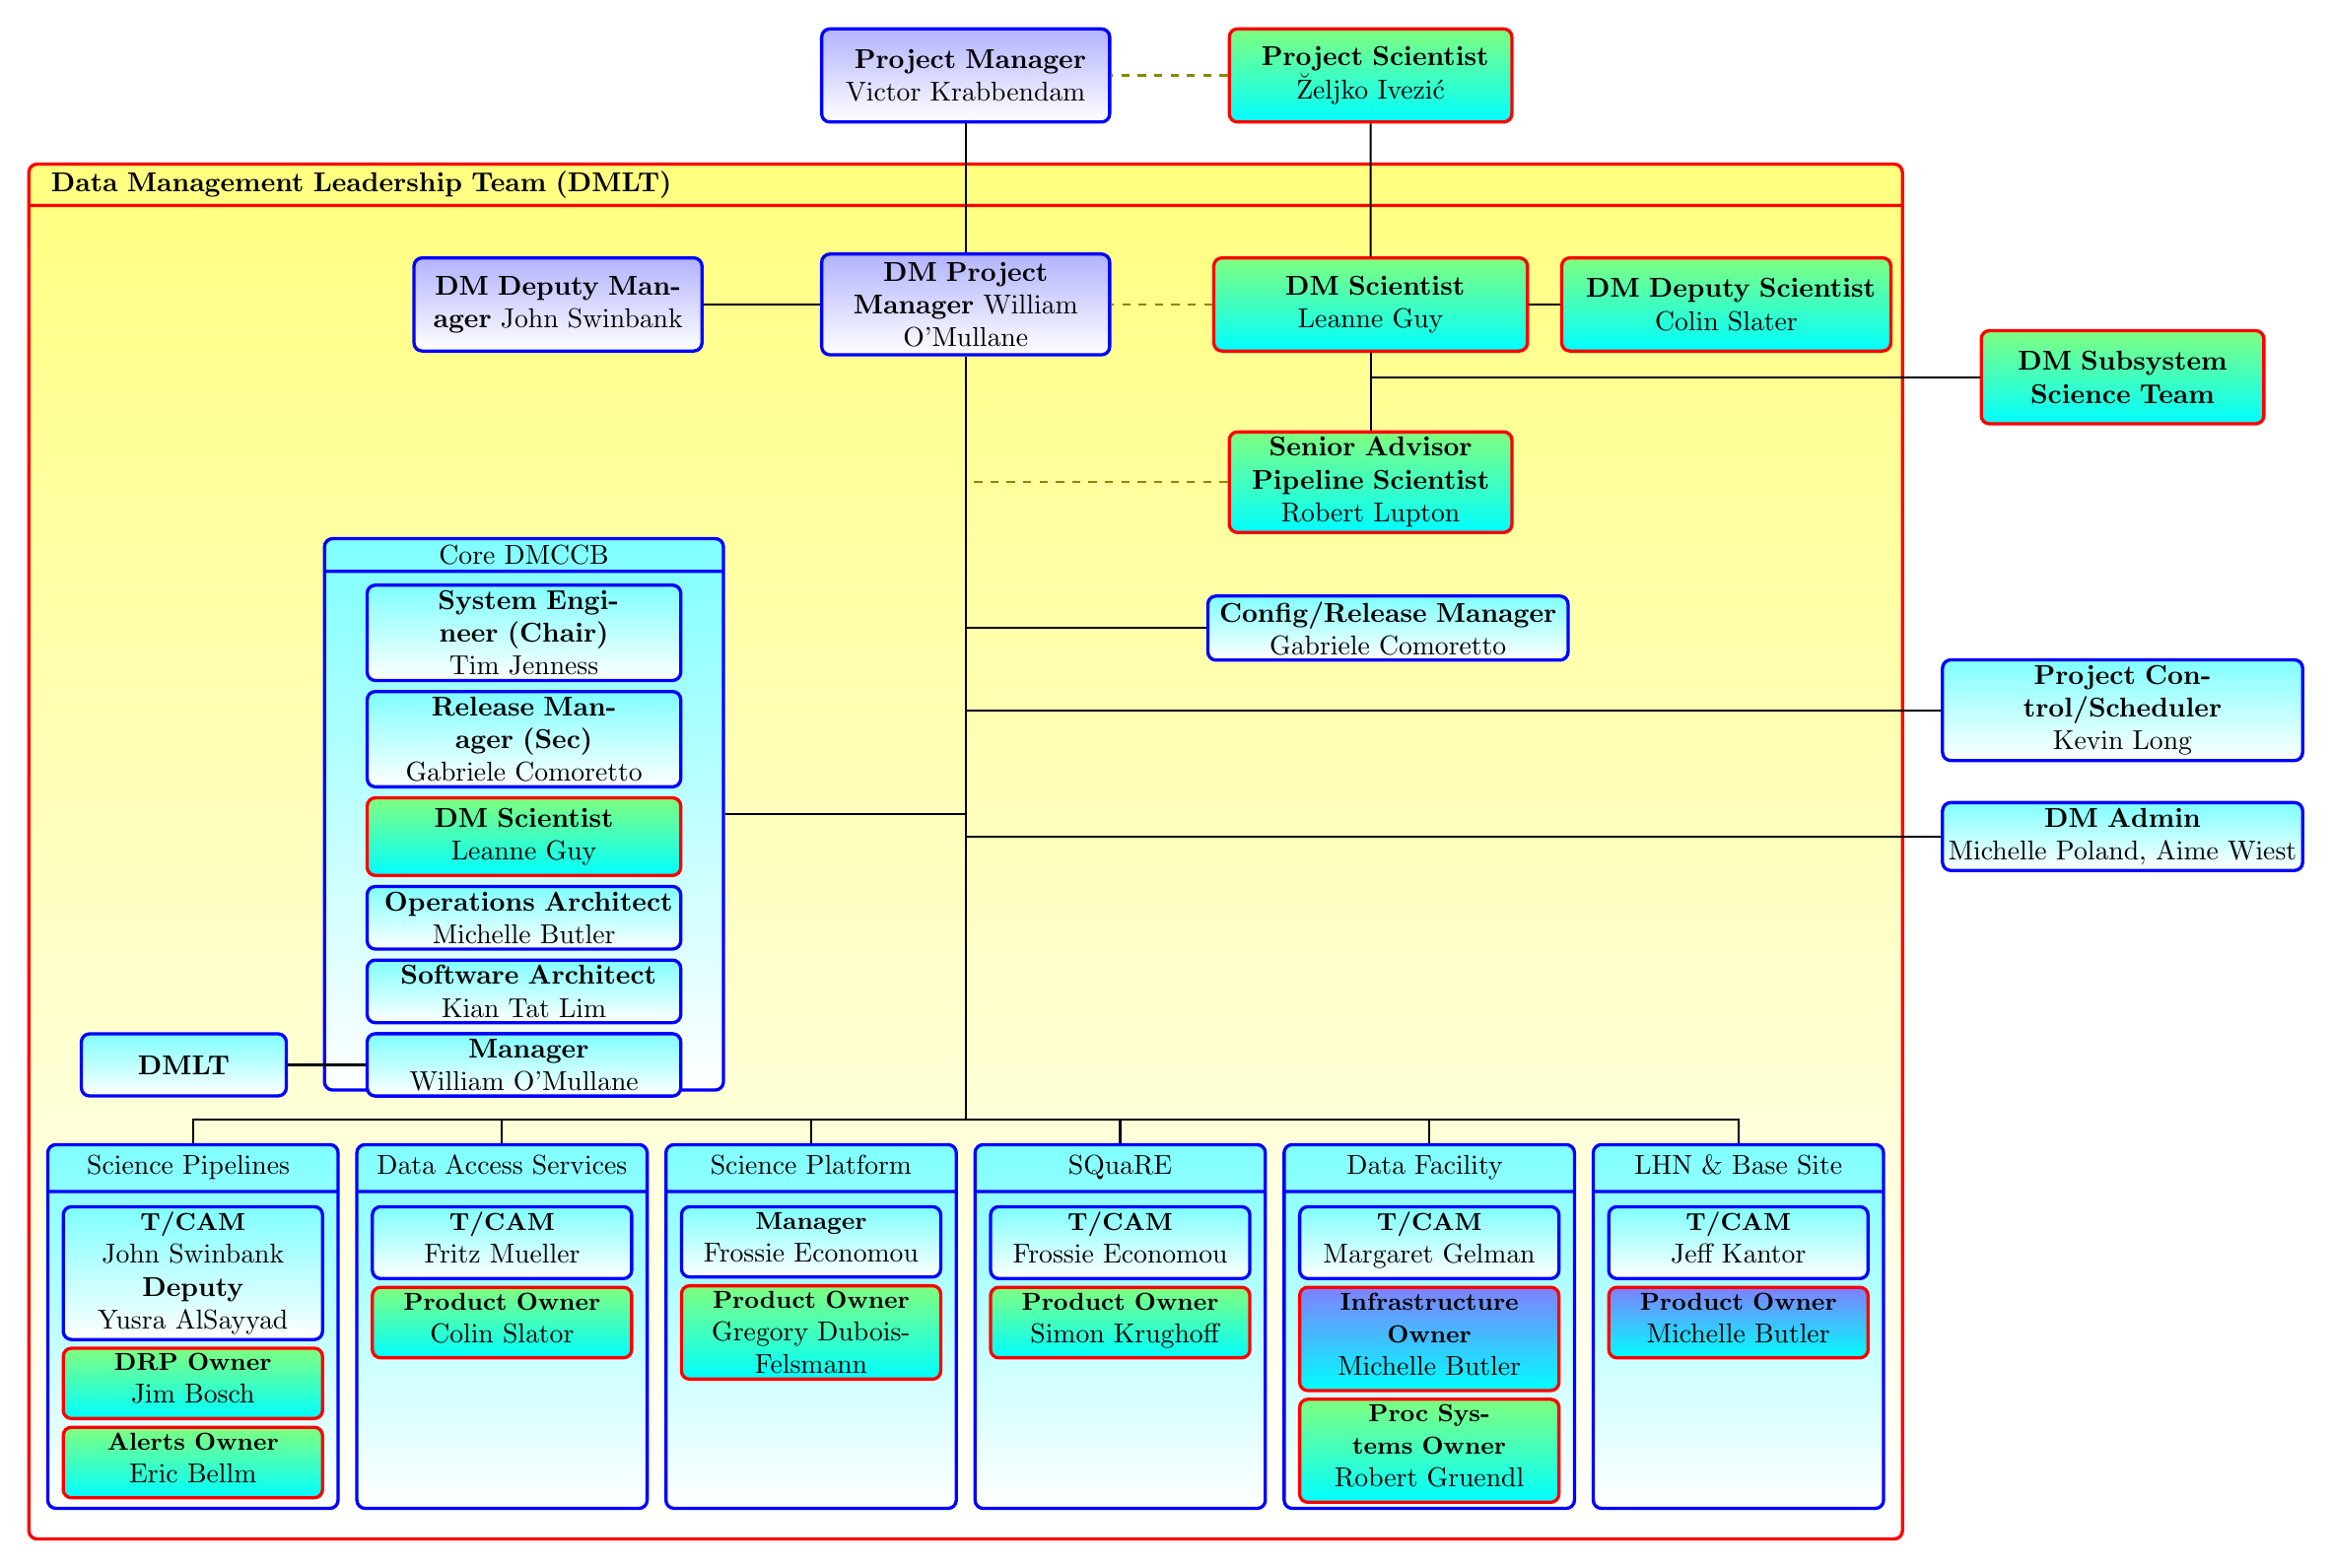
\begin{tikzpicture}[node distance=0mm]


    \node (dm) [arcbox, align=left, text width=24cm,  minimum height=10mm, rectangle split, rectangle split parts=2]
    { \hspace{0.1cm} \textbf{Data Management Leadership Team (DMLT)}
	   \nodepart{second} \vspace{170mm}
	};

    \node (dmpm) [divbox, above=-2.5cm of dm.north] {\textbf{DM Project Manager} William O'Mullane};
    \node (dmdpm) [divbox, left=1.5cm of dmpm] {\textbf{DM Deputy Manager} John Swinbank};
    \node (pm) [divbox, above=.5cm of dm] {\textbf{ Project Manager} Victor Krabbendam};
    \node (dmps) [psbox, right=1.3cm of dmpm, minimum height=12mm, text width=39mm] {\textbf{ DM Scientist}\\ Leanne Guy };
    \node (ddmps) [psbox, right=0.4cm of dmps, minimum height=12mm, text width=41mm] {\textbf{ DM Deputy Scientist}\\ Colin Slater };
    \node (dmadv) [psbox, below=1.0cm of dmps ] {\textbf{Senior Advisor\\Pipeline Scientist}\\ Robert Lupton};
    \node (ps) [psbox, right=1.5cm of pm, minimum height=12mm] {\textbf{  Project Scientist}\\ \u{Z}eljko Ivezi\'c};

    \node (udmpm) [below=59mm of dmpm, text width=0mm]{};
    \node (udmpm1) [below=35mm of dmpm, text width=0mm]{};
    \node (udmpm2) [below=125mm of dmpm, text width=0mm]{};

% SYSENG
            \node (sysengg) [mbox, text width=50mm, rectangle split, rectangle split parts=2, left=3.1cm of udmpm.north]
                {
                 Core DMCCB
                \nodepart{second} \vspace{65mm}
                };
    \node (chair) [mbox, below=6mm of sysengg.north, text width=39mm] {\textbf{ System Engineer (Chair) }\\ Tim Jenness };
    \node (dman) [mbox, below=1mm of chair, text width=39mm] {\textbf{Release Manager (Sec)}\\ Gabriele Comoretto};
    \node (dmsci) [psbox, below=1mm of dman, text width=39mm] {\textbf{DM Scientist}\\ Leanne Guy};
    \node (ops) [mbox, below=1mm of dmsci, text width=39mm] {\textbf{ Operations  Architect}\\ Michelle Butler };
    \node (softarc) [mbox, below=1mm of ops, text width=39mm] {\textbf{ Software Architect}\\ Kian Tat Lim };
    \node (man) [mbox, below=1mm of softarc, text width=39mm] {\textbf{ Manager }\\ William O'Mullane };
%%%% end SYSENG

    \node (cm) [mbox, right=3.1cm of udmpm1.north , text width=45mm] {\textbf{Config/Release Manager }\\ Gabriele Comoretto};
    \node (pconp) [below=5mm of cm] {};
    \node (pcon) [mbox, right=70mm of pconp , text width=45mm] {\textbf{Project Control/Scheduler }\\ Kevin Long};
    \node (admin) [mbox, below=5mm of pcon, text width=45mm] {\textbf{DM Admin}\\ Michelle Poland, Aime Wiest};


    %\node (al) [below=69mm of dmpm, text width=0mm]{};
    \dmmnode[left=1mm of udmpm2.north]{sciplat}{Science Platform}{Frossie Economou}{Gregory Dubois-Felsmann}{psbox} ;
    \dmnode[base left=2mm of sciplat]{das}{Data Access Services}{Fritz Mueller}{Colin Slator} {psbox};

    \node (drp) [mbox, text width=36mm, rectangle split, rectangle split parts=2, base left=2mm of das]
         {Science Pipelines \strut \nodepart{second} \vspace{39mm}};

         \node(drpt) [mbox,minimum height=9mm, below=8mm of {drp}.north, text width=32mm] {\parbox[height=12mm]{0pt}{}{\small \bf T/CAM}\\\strut John Swinbank \\ {\bf Deputy}\\ Yusra AlSayyad };
         \node(drps) [psbox,minimum height=9mm, below=2pt of drpt, text width=32mm] {{\small \bf DRP Owner}\\\strut Jim Bosch};
         \node(alerts) [psbox,minimum height=9mm, below=2pt of drps, text width=32mm] {{\small \bf Alerts Owner}\\\strut Eric Bellm};

	 \dmnode[base right=2mm of sciplat]{square}{SQuaRE} {\strut Frossie Economou}{ Simon Krughoff }{psbox} ;

    \node (infra) [mbox, text width=36mm, rectangle split, rectangle split parts=2, base right=2mm of square]
         {Data Facility \strut \nodepart{second} \vspace{39mm}};

         \node(dft) [mbox,minimum height=9mm, below=8mm of {infra}.north, text width=32mm] {\parbox[height=6mm]{0pt}{}{\small \bf T/CAM}\\\strut Margaret Gelman };
         \node(infrapo) [pobox,minimum height=9mm, below=2pt of dft, text width=32mm] {{\small \bf Infrastructure Owner}\\\strut Michelle Butler};
         \node(procpo) [psbox,minimum height=9mm, below=2pt of infrapo, text width=32mm] {{\small \bf Proc Systems Owner}\\\strut Robert Gruendl};

	 \dmnode[base right=2mm of infra]{lhn}{LHN \& Base Site}{Jeff Kantor}{Michelle Butler}{pobox} ;

 %% GROUPS ..

    \node (dmsg) [psbox, above=3.0cm of pcon, minimum height=12mm] {\textbf{DM Subsystem Science Team}};
    \node (dmlt) [mbox, left=1cm of man.west , text width=25mm] {\textbf{DMLT }};

   \draw[line] (dmps.south) |-  (dmsg.west);
   \draw[line] (dmps.north) --  (ps.south);
   \draw[line] (ddmps.west) --  (dmps.east);
   \draw[line] (dmlt.east) --  (man.west);

   \draw[line] (dmpm.north) -- ++(0,0.8) -| (pm.south);
   \draw[line] (dmdpm.east) --  (dmpm.west);
   \draw[sline] (dmadv.west) -|  (dmpm.south);
   \draw[line] (dmadv.north) --  (dmps.south);

%dm lines second number is the proportional turning point of the line
  % \draw[line] (alerts.north) -- ++(0,0.3) -| (dmpm.south);
   \draw[line] (drp.north) -- ++(0,0.3) -| (dmpm.south);
   \draw[line] (das.north) -- ++(0,0.3) -| (dmpm.south);
   \draw[line] (sciplat.north) -- ++(0,0.3) -| (dmpm.south);
   \draw[line] (square.north) -- ++(0,0.3) -| (dmpm.south);
   \draw[line] (infra.north) -- ++(0,0.3) -| (dmpm.south);
   \draw[line] (lhn.north) -- ++(0,0.3) -| (dmpm.south);

   \draw[line] (sysengg.east) to (udmpm.north);
   \draw[line] (cm.west) -| (udmpm1.north);
   \draw[line] (pcon.west) -| (udmpm1.north);
   \draw[line] (admin.west) -| (udmpm.north);
%science
   \draw[sline] (ps.west) to (pm.east);
   \draw[sline] (dmps.west) to (dmpm.east);


\end{tikzpicture}
\end{document}
